\documentclass[12pt]{article}%
\usepackage{amsmath}%

%\usepackage{bibentry}%
\usepackage{amsfonts}%
\usepackage{amssymb}%
\usepackage{setspace}%
\usepackage{bbm}%
%\usepackage{harvard}
%\usepackage{chicago}
%\bibpunct[,~]{(}{)}{;}{a}{}{,}
\usepackage{enumerate}%
\usepackage{xfrac}
\usepackage[top=1in, bottom=1in, left=1in, right=1in]{geometry}
\usepackage{multirow}
\usepackage{rotating,graphicx}
\usepackage{subcaption}
\usepackage{caption}
\usepackage{rotating}
\usepackage{booktabs}
\usepackage[flushleft]{threeparttable}
\usepackage{subcaption}
\usepackage{float}
\usepackage{appendix}
\usepackage{titletoc}
\usepackage{rotating}



\usepackage[bookmarks=false,colorlinks=true, linkcolor=black, urlcolor=black, citecolor=black]{hyperref}

\usepackage{fullpage}

\usepackage{titlesec}

\usepackage[comma,longnamesfirst]{natbib}%

\newtheorem{hypothesis}{Hypothesis}
\usepackage{xcolor}

\usepackage{xr}

\pdfminorversion=6
\bibpunct[,~]{(}{)}{;}{a}{}{,}
\bibliographystyle{apsr}



\author{Sarah ``Dot" Warren\thanks{Ph.D. student, University of Rochester. Harkness Hall, 333 Hutchinson Rd, Rochester, NY 14627. swarr15@ur.rochester.edu.}}
\title{Who Deserves What, When, and How? Experimental Evidence of Gender Differences in Evaluations of the Deserving Poor\thanks{The experiment reported in this paper is preregistered at EGAP Registry (https://osf.io/u5wxg/). This research was reviewed and approved by the Florida State University Institutional Review Board. All errors remain the author's own responsibility.}}


\date{Draft as of: 3/13/2023}

\begin{document}
\maketitle
\thispagestyle{empty}


\begin{abstract}
While past work clearly demonstrates that women are rewarded less compared to men in the labor market, how do they fare when taking up government aid? I find that, on average, male applicants earn less than female applicants with identical needs. Further, I find the amount awarded to women varies conditional on being rated a ``Poor” or ``Excellent” worker, while there is no difference in the amount awarded to men who are rated ``Poor” workers compared to men who are rated ``Excellent." Thus, women’s advantage over men applicants extends only so far as women are perceived as deserving and hard workers. The totality of these results suggest that people are more inclined to help poor women rather than poor men, but only when the quality of women applicants is validated by an external source. I bolster these findings by providing evidence that neither respondent-level ideology nor gender drives these results.


\end{abstract}
%\vspace{0.5cm}


\newpage


\pagenumbering{arabic}
\begin{doublespace}

The question of ``who should get what, when, and how?" is central to the study of politics \citep{lasswell2018politics}. Understanding this question in a democratic society requires a robust understanding of the public’s answers to these questions and how their values shape their responses. Strategic politicians will not advance redistributive policies for which they believe the public will punish them \citep{fearon1999electoral}. Even outside of the electoral connection, street level bureaucrats are swayed by public opinion. Across many policy areas, including Medicaid \citep{weissert1994beyond}, labor \citep{schmidt2002politicization}, disability insurance \citep{keiser1999state}, food stamps \citep{kogan_welfare_2021}, and immigration \citep{lewis2013some}, street-level bureaucrats use their discretion to align realized policy outcomes with personal and community values, even when their formal responsibility is to implement otherwise identical statutory language. Thus, it is critical that scholars understand how the American public thinks about government aid and its recipients, as scholarship has shown that attitudes about public policies are closely related to attitudes about the beneficiaries of those policies \citep{nelson1996issue, rabinowitz2009white, fossati2018wants}.

The dimension that has characterized past work and public debate on welfare is deservingness \citep{schneider_social_1993, ingram1993constructing, schneider2005deserving,  van2017social, gilens_why_2000, petersen2012social, petersen2012deserves, aaroe2014crowding}. The so-called ``deserving poor” those whose personal financial circumstances have been devastated by structural or macroeconomic forces beyond the individual’s control, rather than personal qualities of dependence and laziness. They are docile and appropriately grateful for the aid they receive, and have or are exerting costly effort to ``earn" assistance \citep{van_oorschot_who_nodate}. For decades, Americans have cared a great deal that aid go only to the most deserving, especially those they feel have earned federal assistance or are particularly helpfuless \citep{bobocel_justice-based_1998, katz_racial_1988, sniderman_symbolic_1986, sniderman_beyond_1996, mclosky_ethos}. But who do Americans think deserves aid from the government? Past work has shown that these deservingness criteria are channels through which Americans express racially biased attitudes \cite{gilens_why_2000}. Welfare attitudes are racialized \citep{desante_working_2013, gilliam_welfare_1999, gilens_why_2000} and programs seen as disproportionately servicing black Americans are viewed significantly less favorably than those servicing white Americans \citep{winter_beyond_2006}, contributing to negative racial stereotypes such as the ``welfare queen."

Yet remarkably little is known about how gender attitudes influence and affect attitudes toward aid recipients. Indeed, much work on gendered attitudes toward welfare recipients considers only attitudes toward men \citep{petersen2012deserves, aaroe2014crowding, willrich2000home} or only attitudes toward women \citep{monnat2010color, desante_working_2013, hayes_2020}, diminishing scholars' ability to make clear, causally identified statements about the role of gender in welfare attitudes. 

In this paper, I address these critical but heretofore unanswered questions by leveraging an original survey experiment to causally identify the effect of gender on perceived deservingness. My analyses show that, when men and women are put in direct competition for scarce public resources, gender-based prejudice interacts with American perceptions of work ethic to amplify existing stereotypes about men and women. I find that, on average, male applicants earn less than female applicants with identical needs. Further, I find the amount awarded to women varies conditional on being rated a ``Poor” or ``Excellent” worker by a third party, while there is no difference in the amount awarded to men who are rated ``Poor” workers compared to men who are rated ``Excellent” workers. Thus, women’s advantage over men applicants extends only so far as women are perceived as ``deserving.” The totality of these results suggest that people are more inclined to help poor women rather than poor men, but only deserving women, when the quality of women applicants is validated by an external source. This research provides evidence toward benevolent sexism, in which women are viewed as weak and in need of extra care \citep{glick_hostile_1997, glick_ambivalent_2001}.

The rest of this paper proceeds as follows. Section I outlines my theory and preregistered hypotheses. Section II details the experimental design. Section III presents the main results. Section IV presents exploratory analyses to confirm that the mechanism driving my results is gender differences in the assigned treatment, rather than respondent covariates. Section V concludes.
\\

\section*{Theory}
Who do Americans think deserves aid from the government? That is, who constitutes the ``deserving poor?" Deservingness tends to operate along five key dimensions: control, need, identity, attitude, and reciprocity. Table \ref{one} provides an overview of these components of deservingness. Different combinations of these criteria often underlie the constructed target populations for federal aid. 

\begin{table}[!h]
	\caption{Dimensions of Deservingness from \cite{van_oorschot_who_nodate}} 
	\label{one}
	\begin{tabular}{l|l}
		\textbf{Dimension}    & \multicolumn{1}{c}{\textbf{Definition}}                                       \\ \hline
		\textit{Control}     & poor people’s control over their neediness, or their responsibility for it    \\
		\textit{Need}        & the level of need                                                             \\
		\textit{Identity}    & the identity of the poor, their proximity to the rich or their ‘pleasantness’ \\
		\textit{Attitude}    & poor people’s attitude towards support, or their docility or gratefulness     \\
		\textit{Reciprocity} & the degree of reciprocation by the poor, or having earned support            
	\end{tabular}
\end{table}

The social construction of target populations refers to the cultural characterizations of people and groups whose behavior are affected by public policy \citep{schneider_social_1993, schneider2005deserving}. These constructs may emerge organically or be developed strategically to influence public opinion of welfare programs or recipients \citep{ingram1993constructing}. \cite{schneider_social_1993} note that federal aid recipients can be grouped into the advantaged or dependent poor. An example of the advantaged poor may be farmers, who receive subsidies even while working hard because they are a powerful and organized interest. Another example of the advantaged poor are the elderly, who have paid into social spending programs for most of their lives and are now collecting hard-earned benefits. Conversely, examples of the dependent poor may be college students or single mothers, who may be subjected to income testing and work-training requirements. These groups may be needier than their advantaged counterparts, but may be less able or have had less opportunities to earn aid. Even while all of these groups may be thought of as members of the ``deserving poor," the social construction of each program's target population paints very different pictures of beneficiaries. While farmers and the elderly fit well with the reciprocity dimension, college students and single mothers may be higher in neediness but less able to reciprocate.

One prominent example of strategic construction is Ronald Reagan's 1976 presidential campaign. The campaign repeatedly referenced Linda Taylor, a black woman who committed welfare fraud, in order to characterize undeserving welfare recipients \citep{gilman2013return}. This, and the publicity surrounding the Taylor affair, led to the construction of the ``welfare queen" stereotype of black women defrauding the government by benefiting from aid while living in luxury. This stereotype is decidedly racialized. Consequently, it is challenging to develop priors on how we should expect it to inform public opinion on women, in general, receiving aid. Indeed, scholarship has consistently found that black women seeking government assistance are evaluated less favorably than otherwise identical white women \citep{gilliam_welfare_1999, desante_working_2013, hayes_2020}.

The racialization of welfare attitudes makes it particularly challenging to evaluate the effect of gender attitudes on evaluations of deservingness \citep{winter_beyond_2006}, because racial and gender attitudes can be difficult to disentangle and may not be additively separable \cite{hayes2021race}. While women receive different treatment than comparable men in everything from applying to jobs \citep{neumark_sex_1996, goldin_orchestrating_2000, quadlin_market} to running for office \citep{hassell_partys_2019, clayton_how_2020} to the price they pay for basic household goods in some countries \citep{betz_womens_2021} to their salaries \citep{castillo_gender_2013, mandel_up_2013}, scholarly intuition is unclear how gender differences in these domains translates into perceptions of deservingness. The prominence and persistence of the welfare queen stereotype suggests that we should perhaps expect women to be evaluated as less deserving, but the racialization of this stereotype suggests that we should not expect that it would apply to non-black women. 

A limited body of empirical work considers how gender might affect perceptions of deservingness \citep{monnat2010color, monnat2010toward}. Women, especially mothers, seeking aid are more likely to be seen as victimized, needy, pleasant, and docile \citep{glick_hostile_1997, glick_ambivalent_2001, schneider_social_1993}, whereas men seeking aid have historically been perceived as failed breadwinners and ``home slackers" \citep{willrich2000home}, in control of their poverty and having not earned aid. Compounding this, Americans have long believed people ``ought to take care of their personal problems by themselves” without relying on the government for aid \citep{sniderman_coping_1977}, yet these values tend to skew toward valuing men's hard work and devaluing men who cannot or do not work \citep{willrich2000home}. Indeed, modern social welfare is often considered a ``women's issue" and welfare policies are favored by women in politics \citep{krook2012all, greene2016diverse}. The combined weight of these attitudes may contribute to public hostility for men receiving public benefits: such policies help those who should be helping themselves \citep{bobocel_justice-based_1998, katz_racial_1988, sniderman_symbolic_1986, sniderman_beyond_1996, mclosky_ethos}.

Given this, I hypothesize:\footnote{All hypotheses and components of the research design were preregistered. My preregistration can be found at: https://osf.io/u5wxg/}

\begin{hypothesis} \label{hyp:first}
	On average, male applicants will be awarded less than female applicants.
\end{hypothesis}

A key dimension on the deservingness literature is applicant quality \citep{petersen2012deserves, petersen2012social}. Applicants perceived as lazy or in control of their poverty are considered less deserving of aid than those who are hardworking and whose financial circumstances are out of their control \citep{aaroe2014crowding}. Because notions of deservingness and undeservingness are frequently characterized by ability and willingness to work, we might think that factors like individual competence will affect perceived deservingness. Specifically, conditional on gender, high competence workers should receive more than their low-competence counterparts.


\begin{hypothesis} \label{hyp:second}
	On average, high-competence applicants will be awarded more than low-competence applicants.
\end{hypothesis}


Deservingness might also be signaled by external factors, such as a college degree, a robust employment record, or participation in a certificate or job training program. If individuals truly prioritize giving aid to good workers whose personal financial circumstances were devastated by forces outside of their control and who they feel have ``earned" assistance, then high-quality workers should be awarded more than low-quality workers. However, scholarship suggests that these kinds of quality evaluations are avenues through which discriminatory attitudes are expressed. For example, \cite{gilens_why_2000} and \cite{desante_working_2013} show that worker quality-based perceptions of deservingness are racialized (e.g. avenues through which respondents express anti-black bias).

The literature on quality evaluations and gender has focused primarily on gender gap reduction in pay, hiring, and promotions. While women in the workforce tend to be penalized for self advocacy \citep{quadlin_market, exley2020knowing}, they tend to benefit disproportionately from external, objective signals of their quality such as GPA \citep{quadlin2018mark}, letters of recommendation \citep{abel_value_2020}, sub-baccalaureate certificates  \citep{dadgar_labor_2015}, and college degrees \citep{jepsen_labor-market_2014}. I therefore hypothesize:


\begin{hypothesis} \label{hyp:thirda}
	For male applicants, there will be no significant difference between amounts awarded to ``Excellent” workers as compared to ``Poor” workers.
\end{hypothesis}

\begin{hypothesis} \label{hyp:thirdb}
	For female applicants, there will be a significant difference between amounts awarded to ``Excellent” workers as compared to ``Poor” workers.
\end{hypothesis}


\section*{Experimental Design and Data}
To test how gender, worker quality, and perceived work ethic shape attitudes toward welfare recipients and the amounts they are awarded, I conducted a survey experiment in which participants were asked to budget money to different pairs of applicants for state assistance subject to a budget constraint. I diverge from past work in which welfare attitudes are elicited in isolation or without budgetary constraints \citep{rabinowitz2009white, aaroe2014crowding, sniderman1993scar, monnat2010color}. Asking participants to make a costly decision is methodologically preferable, because it mitigates concerns about acquiescence bias and is more analogous to real-world decisions in which achieving benefits in one domain may come with costs in another. For example, the 2020 ANES asks respondents whether they think the government should increase spending on services like healthcare and education ``even if it means an increase in spending." That is, given that the government cannot satisfy every need, who deserves to be taken care of first?

I use hand-redacted welfare applications to manipulate targets’ for assistance sex, perceived competence, and objective work-quality rating (Figure \ref{characteristics}). To manipulate quality, each applicant is randomly assigned a worker quality rating of ``Excellent” or ``Poor." To manipulate sex and perceived competence, I use two male and two female names from the \cite{hayes_2020} name-characteristics dataset: Sandra, James, Misty, and Sammie.\footnote{To create the dataset, the authors obtained a list of given names among people born in the United States between the years 1955 and 1990 from the U.S. Social Security Administration (SSA). To identify the gender of the names, they used information on sex included in the SSA data.} These names were specifically selected to minimize the likelihood that factors other than sex, objective, and perceived work ethic would affect treatment. Names are used rather than more overt cues to minimize demand effects \citep{quidt_experimenter_2019, mummolo2019demand}. To mitigate concerns about the effects of race and the racialization of welfare confounding results, all four names chosen were coded as racially distinct white names.

These names are matched on characteristics that Americans report as relevant considerations when evaluating deservingness \citep{bobocel_justice-based_1998, katz_racial_1988, sniderman_symbolic_1986, sniderman_beyond_1996, mclosky_ethos}. Sandra and James are rated highly in professionalism, competence, and work ethic, while Sammie and Misty are rated lower in all three characteristics. Figure \ref{characteristics} below shows the complete breakdown of name-characteristics.

%%NAME CHARACTERISTICS FIGURE HERE
\begin{figure}[h!]
	\centering
	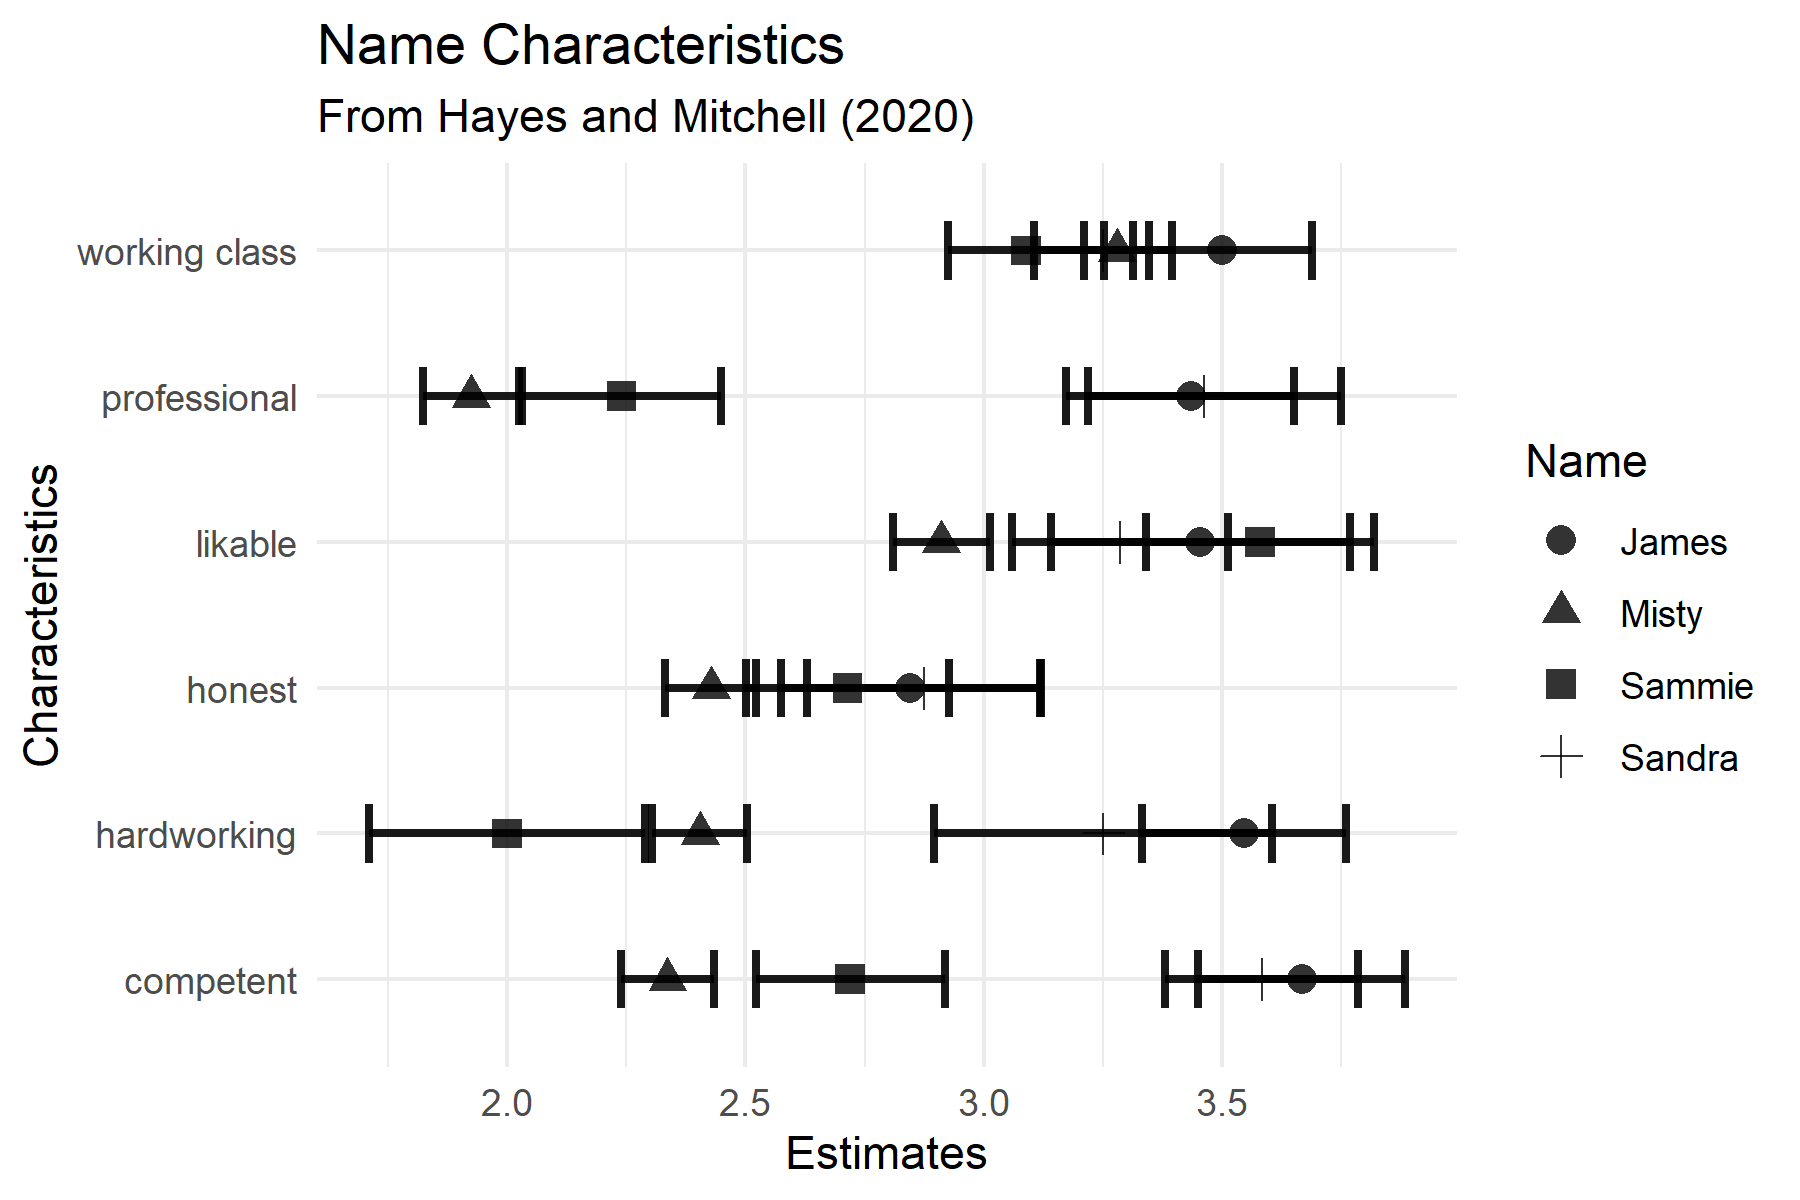
\includegraphics[scale=1]{figs/characteristics.png}
	{\singlespacing
		\parbox{0.75\textwidth}{\scriptsize%\vspace{-0.25cm}
			Takeaway: This figure shows the point estimates and confidence intervals of the estimated valence characteristics of the four chosen treatment names chosen from Hayes and Mitchell (2020). Higher point estimates correspond to higher levels of that value (e.g. a score of 5 in ``professional" corresponds to greater perceived professionalism than a score of 4).
	}}
	\caption{Differences in Valence Characteristics Between Treatment Names}
	\label{characteristics}
\end{figure}

Subjects are given a budgeting task in which they are asked to allocate \$1,500 to two applicants for federal assistance, each of whom has a state-determined need of \$900. Respondents may also choose to give some or all of the funds to ``offset the state deficit.” Participants were given significant discretion in how aid was awarded, constrained only by a budgetary limit and the inability to give an applicant more than their assessed need. Because both applicants’ full need cannot be met, I use the amount awarded to Applicant 1, Applicant 2, and the State as a direct estimate of an applicant’s deservingness. These allocations are my main variables of interest. Everything else about the applicants remains identical, except for a worker quality assessment of Excellent or Poor and their name, which cues both sex (male or female) and competence (high or low). If an applicant receives a different allocation across treatments, we can infer that this difference is due to experimental manipulation. Further, as the applicant’s characteristics were manipulated via random assignment, \textit{any} difference in the relative importance respondents place on fiscal responsibility—illustrated by giving more to offset the budget deficit—can also be traced back to the experimental treatment. 

Having the option to allocate dollars to a non-aid resource (in this case, the budget deficit) allows me to separate gender-neutral values from gendered discrimination. This deficit option also allows for individuals to take a principled position, a socially desirable and available option, to decide that the money would be better spent in some other way. While it may be the case that some respondents chose to allocate dollars to the state out of principled objection, whereas others believe that deficit reduction is simply a higher priority, both are a function of gender-neutral policy positions and should have no bearing on the \textit{difference between} the amounts awarded to the baseline and treatment applicants.

%%SAMPLE APPLICATIONS FIGURE HERE
\begin{figure}[h!]
	\centering
	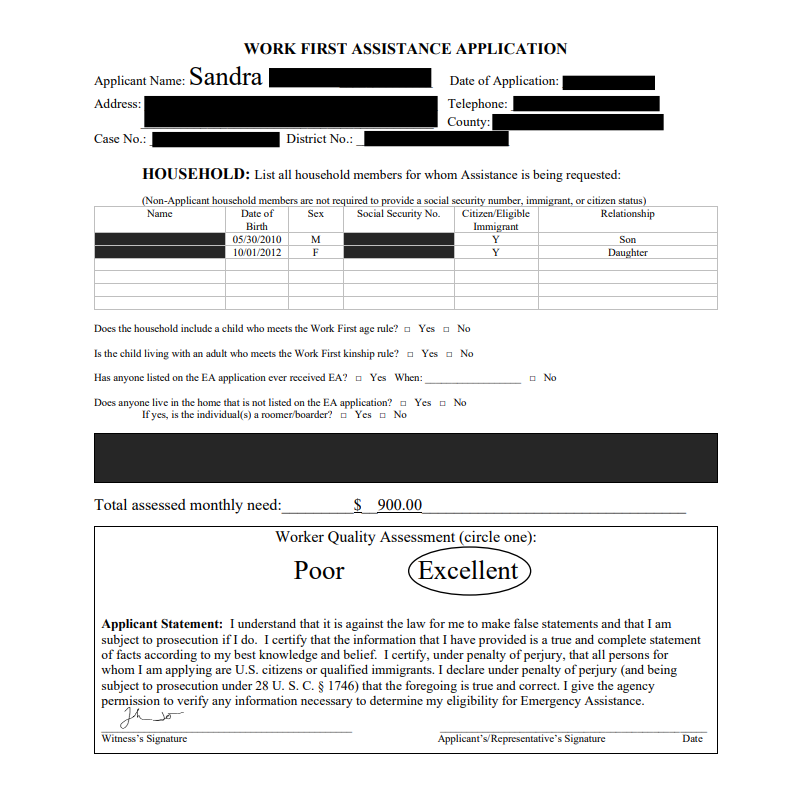
\includegraphics[scale=1]{figs/example_treatment.png}
	\caption{Example Aid Application}
	\label{figure2}
\end{figure}


In order to isolate the effects of sex versus the traits people ascribe to different names, I fielded a survey experiment with YouGov (n=1880) in April 2022. The sample is a mixture of a nationally representative sample with a low socio-economic status oversample. Due to this, in interpreting my results, I focus on effect direction, rather than magnitude, though I report point estimates in all cases \citep{horton2011online}.\footnote{I present the same analysis conducted on the nationally representative and low-SES subsamples in Appendix A.} 

Respondents viewed two applications identical in appearance except for the realized treatment conditions. Rather than randomizing both applications, all respondents viewed the same baseline application of ``Sandra” who was rated as ``Excellent” compared to a second application. I used a 2x2x2 factorial design for this second application, randomizing sex (male/female), competence (high/low), and quality assessment (excellent/poor) of the second application, using the names James, Misty, and Sammie as my cue for sex and competence. Respondents were then asked to allocate funding to the two applicants or to offset the state budgetary deficit.

\section*{Experimental Results}
When men and women are put in direct competition for scarce resources, how do women fare compared to similarly-situated men? How does perceived competence and external quality ratings affect this relationship? Figure \ref{results-main} presents the main results of the experiment by treatment name, with color denoting the quality rating (Excellent/Poor) of the treatment name, and point-shape denoting the amount given to each recipient. Recall that the baseline condition is an applicant named Sandra, a high-competence name, who is rated as an ``Excellent” quality worker.

%%MAIN RESULTS FIG HERE
\begin{figure}[h!]
	\centering
	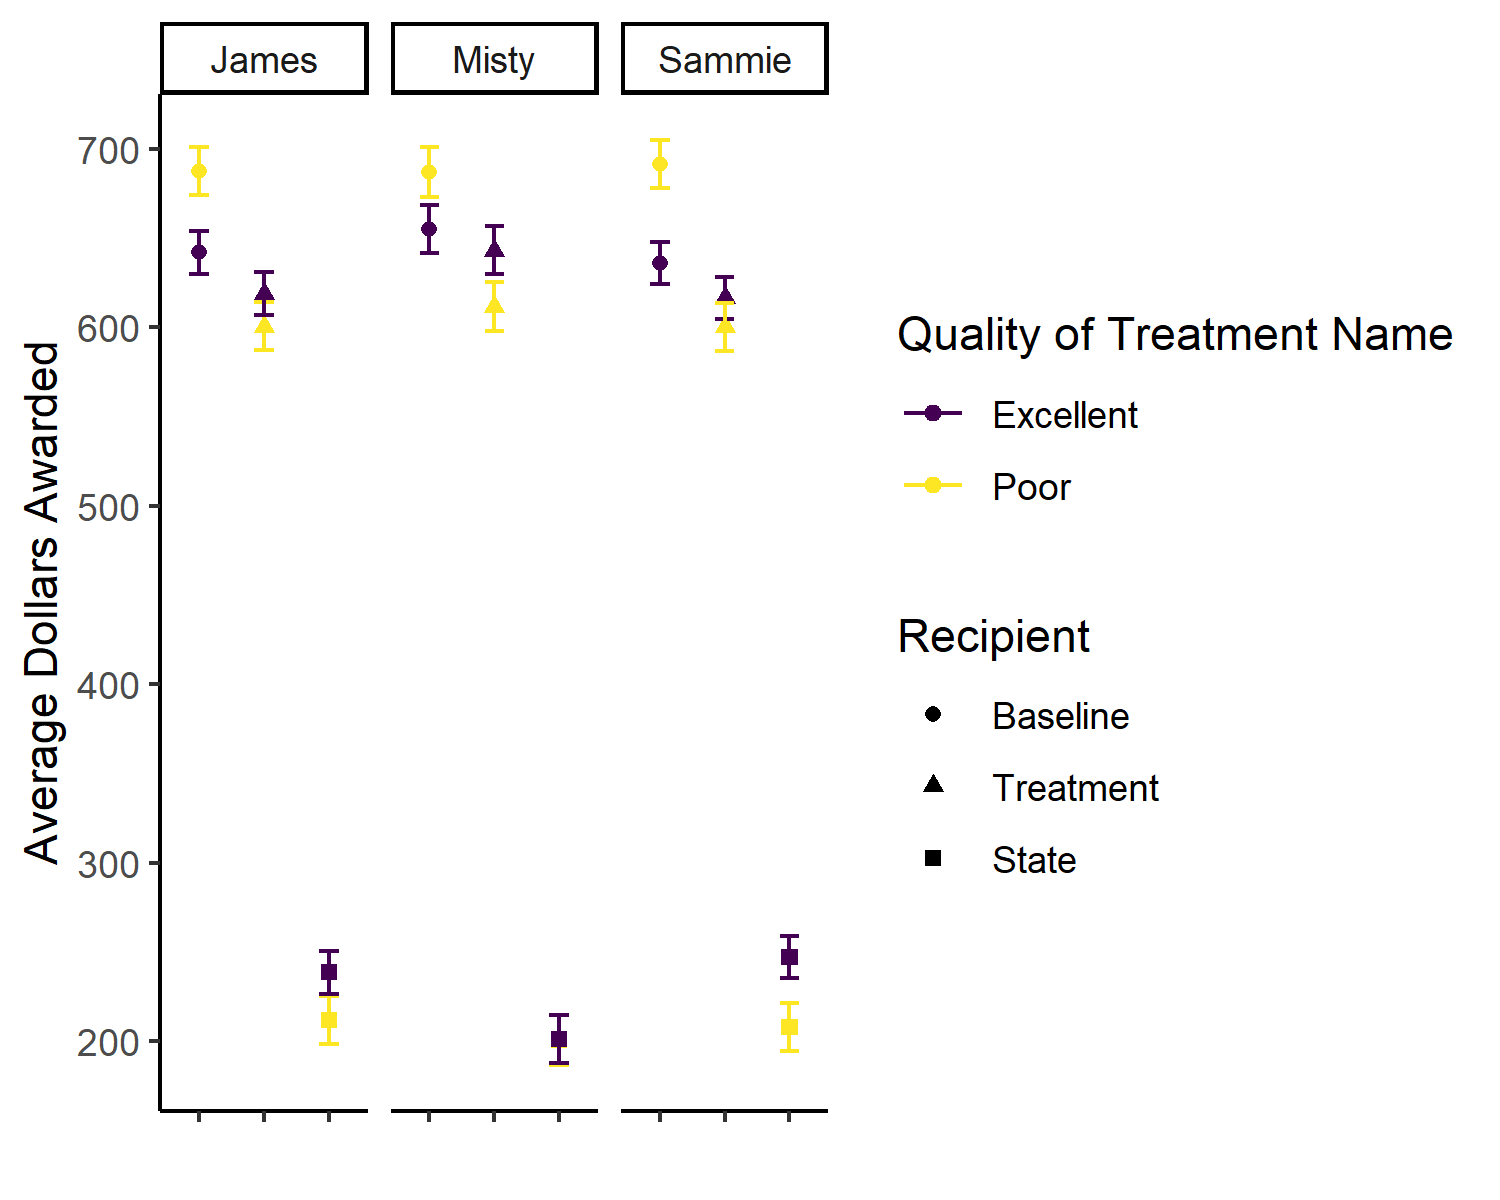
\includegraphics[scale=1]{figs/general-results-name.png}
	{\singlespacing
		\parbox{0.75\textwidth}{\scriptsize%\vspace{-0.25cm}
			Takeaway: This figure shows the results for each treatment condition. The y-axis is the average dollars awarded to each possible recipient (the baseline, the treatment, or the state). The x-axis is each possible recipient (the baseline, the treatment, or the state). This allows us to compare the treatment to the baseline in each condition, as well as the treatment name to itself when the quality rating is manipulated. Error bars are 95\% confidence intervals.
	}}
	\caption{Gender Differences in Aid Allocated by Treatment Name}
	\label{results-main}
\end{figure}

H1 predicts that, on average, male applicants will be awarded less than female applicants. The first panel of Figure \ref{results-main} demonstrates that, when she is paired with a high-competence, ``Excellent” male name, James, Sandra is awarded significantly more on average (\$642.06 vs. \$619.20, p = 0.014). \footnote{Excellent Sandra also earns more on average than Sammie, a low-competence name, when he is rated ``Excellent” (\$635.98 vs \$616.60, p=0.000).} However, there is also no significant difference between Excellent Sandra and Excellent Misty (\$655.31 vs \$643.20, p=0.141). These results are consistent with H1, in that Excellent Misty earns no less than Excellent Sandra, while Excellent James earns substantively and significantly less than the baseline.

Turning to competence, I consider the difference between name valence characteristics and aid amounts awarded. Recall that competence is determined by valence-characteristic scores in the Names Dataset \citep{hayes_2020}. Hayes and Mitchel’s findings suggest that name-characteristics have the potential to minimize differences in aid allotment due to racial prejudice; however, the mitigating effects of name-characteristics do not appear to extend to gender bias. Sandra and James are both high-competence names, while Misty and Sammie are relatively low-competence. I predicted in H2 that high competence names should receive more, on average, than low competence names. Thus, holding applicant quality constant, Sandra should receive more than Misty and James should receive more than Sammie, relative to the baseline. I do not find empirical support for H2. There is no statistically or substantively significant difference between the amounts awarded to Excellent Misty and Excellent Sandra (\$655.31 vs \$643.20, p=0.141), nor is there between Excellent James and Excellent Sammie (\$619.20 and \$616.60, p=0.88), and Poor James and Poor Sammie (\$600.60 and \$600.32, p=0.986). This suggests that, among whites, perceived competence may matter less than when making inter-racial comparisons.

Finally, I predicted that, for male applicants, there will be no significant difference between amounts awarded to workers rated ``Excellent” as compared to workers rated ``Poor.” Conversely, I predicted that the opposite will be true for female applicants; that is, worker quality rating will result in a significant difference in the amount awarded. To evaluate H3 and H4, I compare the difference in means for each treatment name to (James, Sammie, and Misty) when they are ``Excellent” rated workers to when they are rated ``Poor.” Table \ref{lasttable} shows the results of this test, which support H3 and H4. There is a statistically significant difference in the amount of aid awarded to Excellent Misty compared to Poor Misty; however, there is no such difference between Excellent Sammie or James compared to Poor Sammie or James.

\begin{table}[!htbp] \centering 
	\caption{The Effect of Quality on Deservingness} 
	\label{lasttable} 
	\footnotesize 
	\begin{tabular}{@{\extracolsep{1pt}} ccccccc} 
		\\[-1.8ex]\hline \\[-1.8ex] 
		& Condition & Mean 1 & Mean 2 & Upper CI & Lower CI & p-value \\ 
		\hline \\[-1.8ex] 
		& Excellent Misty vs Poor Misty & 643.198 & 611.797 & 0.728 & 62.073 & 0.045** \\ 
		 & Excellent James vs Poor James & 619.198 & 600.589 & -13.564 & 50.781 & 0.256 \\ 
		 & Excellent Sammie vs Poor Sammie & 616.598 & 600.317 & -18.015 & 50.576 & 0.352 \\ 
		\hline \\[-1.8ex] 
	\end{tabular} 
\end{table} 


The totality of these results suggest that identically-situated men and women are evaluated differently when put in competition for scarce resources. Though implicit competence does not appear to play a role in aid evaluations when comparing white men and women to each other, positive third-party quality ratings affect women’s earnings and do not alter men’s.

\section*{Evaluation of the Mechanism\footnote{Exploratory analysis. The following analysis was not part of my pre-registration plan.}}
I theorized that perturbing the gender of applicants is the sole cause of changes in the dollar amounts awarded to applicants and took special care to allow participants to have a socially desirable channel to express gender-neutral, value-based sentiment. Still, public aid is a partisan policy position. Historically, liberal voters and politicians favor more robust public aid programs, where as conservatives tend to oppose them. It could be the case that partisanship is driving both gender-based attitudes \textit{and} attitudes towards welfare. Further, it may be the case that survey participants' are a function of in-group attitudes. That is, if female respondents award more to female applicants and male respondents award more to male applicants, my results may not be a function of gender attitudes, but simply a function of receiving a treatment condition in one's in-group compared to one's out-group.

To bolster confidence that the mechanism driving my results is varying applicants' gender and not other factors, like respondents' ideology or in-group favoritism, in this section I perform a series of tests for heterogeneous treatment effects by respondent ideology and gender.

\subsection*{Ideology}
To mitigate concerns about respondent ideology driving my results, I compare the difference in the amount given to the baseline and the treatment name across self-reported ideology. First, I check whether there is a difference in the differences between the baseline and excellent-rated Misty between ideologies. If ideology, rather than gender, is driving my results, we should see statistically significant differences in the differences between the treatment and baseline, regardless in the overall magnitude of the results. In other words, even if conservative respondents give less, on average, to both applicants due to a principled objection to public aid, the \textit{difference} in the amount given to Excellent Misty and the amount given to Excellent Sandra should not vary \textit{unless} ideological differences are driving my results. Table \ref{ideo-mist} shows the results of unpaired t-tests across ideological self-identifications. The differences in the differences is statistically indistinguishable from zero across ideologies.

\begin{table}[!htbp] \centering 
	\caption{Ideological Differences in Excellent Misty Treatment} 
	\label{ideo-mist} 
	\begin{tabular}{@{\extracolsep{5pt}} cccccc} 
		\\[-1.8ex]\hline 
		\hline \\[-1.8ex] 
		& Group 1 & Group 2 & $n_{Group 1}$ & $n_{Group 2}$ & p \\ 
		\hline \\[-1.8ex] 
		& Very Conservative & Conservative & 42 & 57 & 0.867 \\ 
		 & Very Conservative & Moderate & 42 & 102 & 0.506 \\ 
		 & Very Conservative & Liberal & 42 & 49 & 0.82 \\ 
		 & Very Conservative & Very Liberal & 42 & 35 & 0.607 \\ 
		 & Conservative & Moderate & 57 & 102 & 0.446 \\ 
		 & Conservative & Liberal & 57 & 49 & 0.922 \\ 
		 & Conservative & Very Liberal & 57 & 35 & 0.417 \\ 
		 & Moderate & Liberal & 102 & 49 & 0.509 \\ 
		 & Moderate & Very Liberal & 102 & 35 & 0.207 \\ 
		 & Liberal & Very Liberal & 49 & 35 & 0.388 \\ 
		\hline \\[-1.8ex] 
	\end{tabular} 
\end{table} 

Next, I examine whether there is a difference in the differences between the baseline and excellent-rated James between ideologies. As before, if ideology is driving my results, there should be statistically significant differences in the differences from baseline between ideologies, because respondents with different ideologies are behaving differently. Table \ref{ideo-james} shows the results of unpaired t-tests across ideological self-identifications. The differences in the differences is once again indistinguishable from zero across ideologies.

\begin{table}[!htbp] \centering 
	\caption{Ideological Differences in Excellent James Treatment} 
	\label{ideo-james} 
	\begin{tabular}{@{\extracolsep{5pt}} cccccc} 
		\\[-1.8ex]\hline 
		\hline \\[-1.8ex] 
		& Group 1 & Group 2 & $n_{Group 1}$ & $n_{Group 2}$ & p \\ 
		\hline \\[-1.8ex] 
		 & Very Conservative & Conservative & 36 & 43 & 0.89 \\ 
		 & Very Conservative & Moderate & 36 & 101 & 0.917 \\ 
		 & Very Conservative & Liberal & 36 & 52 & 0.987 \\ 
		 & Very Conservative & Very Liberal & 36 & 41 & 0.621 \\ 
		 & Conservative & Moderate & 43 & 101 & 0.95 \\ 
		 & Conservative & Liberal & 43 & 52 & 0.876 \\ 
		 & Conservative & Very Liberal & 43 & 41 & 0.722 \\ 
		 & Moderate & Liberal & 101 & 52 & 0.9 \\ 
		 & Moderate & Very Liberal & 101 & 41 & 0.568 \\ 
		 & Liberal & Very Liberal & 52 & 41 & 0.485 \\ 
		\hline \\[-1.8ex] 
	\end{tabular} 
\end{table} 

\subsection*{In-Group Favoritism}
Finally, I consider whether respondent's gender could be accounting for the results I observe. Extant work shows that individuals are more generous to members of their in-group \citep{chen2009group}. If respondents respond heterogeneously to the treatment based on whether the treatment they receive matches their gender, we should expect to see differences in the amounts male and female respondents allocate to Misty and James. Table \ref{gender} shows the results of an unpaired t-test between male and female respondents on the differences from baseline in the Excellent Misty and Excellent James condition. There are no statistically significant differences.

\begin{table}[!htbp] \centering 
	\caption{Gender Differences in Differences from Baseline} 
	\label{gender} 
	\begin{tabular}{@{\extracolsep{5pt}} ccccccc} 
		\\[-1.8ex]\hline 
		\hline \\[-1.8ex] 
		& Group 1 & Group 2 & $n_{Group 1}$ & $n_{Group 2}$ & p & Treatment Name \\ 
		\hline \\[-1.8ex] 
		 & Female & Male & 187 & 126 & 0.723 & Excellent Misty \\ 
		 & Female & Male & 164 & 134 & 0.742 & Excellent James \\ 
		\hline \\[-1.8ex] 
	\end{tabular} 
\end{table} 

Given these results, we can be quite confident that the results are not simply a function of respondent's ideology or in-group favoritism, but are in fact due to experimental manipulation eliciting attitudes about male and female aid applicants.

\section*{The Caustic Effect of Gender Stereotypes}
This article addresses a fundamental question concerning American's political attitudes toward government redistribution: Does gender matter? Qualitative and historical scholars posit a strong link between gender and deservingness, and empirical research exploring the consequences of perceived deservingness often draws heavily on this normative literature. At the same time, gender and politics scholarship largely focuses on differences in perceived deservingness within men and women or within racial groups. Less attention has been dedicated to examining how gender attitudes influence American's attitudes toward welfare recipients. My work fills this gap by providing a theoretical framework and experimental tests that illuminate the link between gender, American values, and deservingness.

I find that gender and American values of hard work jointly influence how individuals evaluate the deserving poor. To begin, my results suggest that, on average, women are perceived as more deserving than similarly situated men. This is in line with historical and qualitative scholarship \cite{willrich2000home} and broadly suggestive of ambivalently sexist attitudes in the public \citep{glick_ambivalent_2001, glick_hostile_1997}. Moreover, I find that third-party quality evaluations yield higher dividends for women, whereas they yield no effects for men. This result comports with a large body of scholarship suggesting that, absent external interventions, women's abilities and contributions are taken less seriously than their male counterparts. One solution identified by scholars across disciplines for helping disadvantaged women overcome these hurdles is additional job training and certificate programs that provide an external, reliable evaluation of their quality as a worker \citep{abel_value_2020, dadgar_labor_2015, jepsen_labor-market_2014}. My results suggest that these kinds of interventions are likely to improve the outcomes of women applying for aid, but not men. As a point of departure from past scholarship on the realization of welfare attitudes \citep{hayes_2020}, I find that the valence characteristics of treatment names has no effect on the amount awarded applicants.

Moreover, my experimental methodology serves as a point of departure for a much broader research agenda. By imposing a budgetary constraint, I am able to avoid acquiescence bias and put respondents in a decision-making environment which more closely mirrors the real world. In so doing, I am better able to answer the question: given that the government cannot satisfy every need, who should it take care of first? Protecting women, especially those who are good workers, appears to be the foremost priority. One implication of this result is that policymakers are most likely to garner support for government aid programs when their messaging about these programs is focused on how they will support hardworking women, such as single mothers. Further work is needed to understand how the gender attitudes reported here extend into political messaging and policy evaluations.

Future work would also benefit from a more robust understanding of why good female workers, in particular, are favored, as this seems to cut against notions of ambivalent sexism, in which women fulfilling traditional, home-bound duties are praised and protected and those failing to do so are punished. Additionally, future work should consider what can be done in the fact of gender differences in deservingness between otherwise identical applicants. If the normative goal is an equitable society, then presumably the normatively best result is one in which there are no differences between a ``Sandra" or a ``James", holding all else constant. This work raises clear questions as to what additional measures will reduce the gender differences in perceived deservingness of applicants. In this way, my work lays the foundation for additional research on the American welfare state.

\end{doublespace}

\pagebreak

\bibliography{womenref}


\end{document}
